% THIS IS AN EXAMPLE DOCUMENT FOR VLDB 2012
% based on ACM SIGPROC-SP.TEX VERSION 2.7
% Modified by  Gerald Weber <gerald@cs.auckland.ac.nz>
% Removed the requirement to include *bbl file in here. (AhmetSacan, Sep2012)
% Fixed the equation on page 3 to prevent line overflow. (AhmetSacan, Sep2012)

\documentclass{vldb}
\usepackage{graphicx}
\usepackage{balance}  % for  \balance command ON LAST PAGE  (only there!)
\usepackage{color}

\begin{document}

% ****************** TITLE ****************************************

\title{Two Phase Commit on Persistent Key Value Store with Data Replication}

% possible, but not really needed or used for PVLDB:
\subtitle{6.824 Distributed Systems Final Project}
%\titlenote{A full version of this paper is available as\textit{Author's Guide to Preparing ACM SIG Proceedings Using \LaTeX$2_\epsilon$\ and BibTeX} at \texttt{www.acm.org/eaddress.htm}}}

% ****************** AUTHORS **************************************

% You need the command \numberofauthors to handle the 'placement
% and alignment' of the authors beneath the title.
%
% For aesthetic reasons, we recommend 'three authors at a time'
% i.e. three 'name/affiliation blocks' be placed beneath the title.
%
% NOTE: You are NOT restricted in how many 'rows' of
% "name/affiliations" may appear. We just ask that you restrict
% the number of 'columns' to three.
%
% Because of the available 'opening page real-estate'
% we ask you to refrain from putting more than six authors
% (two rows with three columns) beneath the article title.
% More than six makes the first-page appear very cluttered indeed.
%
% Use the \alignauthor commands to handle the names
% and affiliations for an 'aesthetic maximum' of six authors.
% Add names, affiliations, addresses for
% the seventh etc. author(s) as the argument for the
% \additionalauthors command.
% These 'additional authors' will be output/set for you
% without further effort on your part as the last section in
% the body of your article BEFORE References or any Appendices.

\numberofauthors{2} %  in this sample file, there are a *total*
% of EIGHT authors. SIX appear on the 'first-page' (for formatting
% reasons) and the remaining two appear in the \additionalauthors section.

\author{
% You can go ahead and credit any number of authors here,
% e.g. one 'row of three' or two rows (consisting of one row of three
% and a second row of one, two or three).
%
% The command \alignauthor (no curly braces needed) should
% precede each author name, affiliation/snail-mail address and
% e-mail address. Additionally, tag each line of
% affiliation/address with \affaddr, and tag the
% e-mail address with \email.
%
% 1st. author
\alignauthor
Xiangyao Yu\\
       \affaddr{Massachusetts Institute of Technology}\\
       \affaddr{32 Vassar Avenue}\\
       \affaddr{Cambridge, MA}\\
       \email{yxy@mit.edu}
% 2nd. author
\alignauthor
Shuotao Xu\\
       \affaddr{Massachusetts Institute of Technology}\\
       \affaddr{32 Vassar Avenue}\\
       \affaddr{Cambridge, MA}\\
       \email{shuotao@mit.edu}
}


\maketitle

\begin{abstract}
  We implemented a distributed transaction processing system where data is
  partitioned and mapped to different shards. All shards are replicated to enhance
  the availablity and durability of the system. The database model is simple
  key-value store inherited from Lab 4. The objectives of the project are 1) to
  process transaction using two phase commit and guarantee atomic execution, 2) to
  persistently store data and server status on disk to tolerate server failures in
  time of reboot. The requests of a transaction consist of GET, PUT, and ADD. To
  simplify implementation, the only scenario of abort of a transaction is that it has
  an add request that results a negative value. Firstly, we implemented a
  coarse-grained locking scheme where a transcation locks the groups it
  touches. Secondly, We implemented test cases to verify the correctness of the
  system under different failure scenarios including unreliable networks and server
  failures. Then we benchmarked our system with synthetic workloads that varies with
  parameters like read/write ratios of a transcation, number of clients and so
  on. Lastly, in order to achieve better performance gains, we refined our system
  with a fine-grained locking scheme where a transcation locks the keys it touches.
\end{abstract}


%\section{Introduction}

%foo


\section{Implementation Details}

Our persistent key value store is constructed such that each key of type string is
mapped to a value of type integer. We confined the type of values to integer to allow
arithmetic operations on the key-value pairs. The data of our systems are partitioned
into different shards. A group of servers are responsible for a distinct subset of
shards, and all data within a group are replicated. Our system supports atomic
transcation, where a transcation is an ordered group of requests such as puts, gets
and etc. We also support persistency, where all commited transcations are recorded to
disk. Our persistent key-value store is useful such that it could be a high
performance inventory management system.

\subsection{Transcation Support}

Our system supports transcation consisting of requests of PUTs, GETs, and ADDs.
\begin{itemize} 
\item a PUT updates the value associated with the key
\item a GET returns the value associated with the key
\item an ADD adds a value (could be negative) to the previous value associated with
  the key
\end{itemize}

In particularly, the transcation support of our system ensures the following properties. 

\textbf{Consistency} Our system allows multiple clients to send transcations
concurrently. Specifically, our database enforce seqential consistency such that the
effects of concurrent transcations appears as some seqential order. To enable
seqential consistency, the client should lock the groups that a transcation touches
before execuation. And since we will have multiple servers within each group, we will
ensure consistency inside the group with Paxos, to guarantee a global ordering of the
operations within a group.

\textbf{Atomicity} The transcations need also be atomic, i.e. either all of the
requests of the transcation are executed or none are executed. We ensure atomicity of
the transcation with two phase commit protocol.

\textbf{Persistency} All the effects of a committed transcation on key value store
are written on disk.

\textbf{Fault-tolerant} Our system ensures the transcation processing is
fault-tolerant. On the server sides, the Paxos implementation in Lab 3 has already
ensured tolerance under network failures. In our project, we will modified Lab 3 such
that Paxos can also handle server crashes. On client side, we will also record its
transcation processing status on disk, so that after crash, the client will know at
which point it was processing the transcation.

\subsubsection{Persistent Paxos}

We made the Paxos persistent so that it can tolerate server crash.

Whenever any of the propose numbe(n\_p), accepted number(n\_a) and accepted value(v\_a)
is modified, all of them are written to the file system with the file name in the
following format: \textit{SERVERNAME\_INS\#.txt}.

When the paxos log is truncated, the corresponding files are also deleted. When a
server reboots after failure, it will reconstruct the Paxos instances by reading from
the file system. We use a lazy reconstruction approach where an instance is read and
reconstructed only when it is touched.

Moreover, we added a new function call, Poll(seq int), to the Paxos, to peek the
status of a Paxo instance at some sequence number. When Poll(seq int) is called, the
paxos server first checks locally if the Paxos instance of sequence num \textit{seq}
has been decided (by calling Status()). If not, RPCs are sent to peer servers and the
status of the instance is returned. Note that Poll() is different from Status() since
Status() only checks the Paxos instance on local server.

Poll is used to check whether a particular instance has been decided. This simplifies
our system implementation as explained in Section~\ref{?sec:2pc}.


\subsubsection{Locking Scheme}
\label{sec:lock}

We uses locking to ensure seqential consistency of concurrent transcations.

Transactions are initiated at the client side. A client breaks down a transcation,
and sends the requests to a server in the corresponding group. Upon receiving the
requests, the server will start a paxos instance to agree on the transcation. This
paxos instance locks the whole group for the transaction.

To avoid deadlocks, the clients should send requests to the groups sequentially
following a fixed order, such as the order of increasing group IDs.

To tolerate failures, we have Paxos handle failures on server side. On client side,
when a transcation starts, the client will record its status as \textit{started} on
disk. When all groups are properly locked, the on-disk status of the client changes
to \textit{locked}.

This is the first step of transcation processing from client's perspective, we call
it \textit{insert transcation}.


\subsubsection{Two Phase Commit}
\label{sec:2pc}

After client hears from all groups that the servers have been properly locked for the
transcation, it initializes two-phase commit(2pc) protocol as described in Figure
\ref{fig:2pc}, where the records with * are written into non-volatile storage.

\begin{figure}[h!]
  \centering
  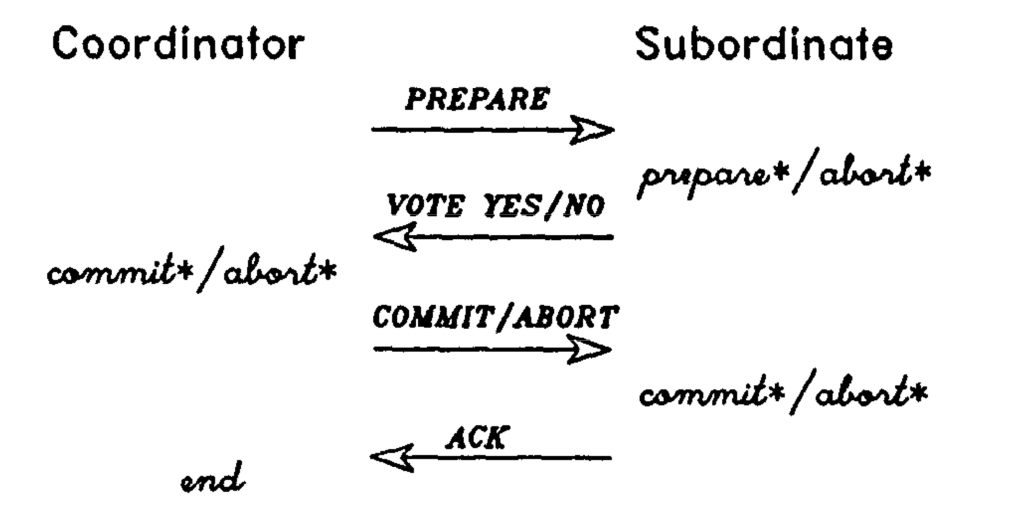
\includegraphics[width = 0.8\linewidth]{figs/2PC.pdf}
  \caption{Two Phase Commit Protool}
  \label{fig:2pc}
\end{figure}

The client will first send prepare messages to all the groups that a transcation
involves in parallel to make sure the transcation can be executed. The servers
pre-run the transcation. And if there is an ADD request that results negative
interger, it responses abort. Otherwises, the server responses prepare\_ok. The
client waits for all prepare responses from different groups. And depends on the
prepare messages, client 1) sends out reply to application and 2) either sends out
commit or abort message to servers. After servers sees commit, it will write the
result of the transcation into persistent storage.

As shown in Figure \ref{fig:2pc}, two-phase commit requires the coordinator(client)
to write once to the persistent storage (commit/abort) and subordinate(servers) to
write twice to the persistent storage (prepare\_ok/abort and commit/abort). In our
implementation, the server always need to make consensus on those two messages
through Paxos. Since our paxos is already persistent, two phase commit is
automatically achieved at the server side. 

At the client side, we added an extra disk operation to make the state of the current
transaction persistent. When a client reboots, it will first read the disk for the
latest state before it crashed and repeat the last operation if necessary. 

The servers, on the other hand, should either passively wait for the client’s
requests to insert Paxo instance. So it does not have to recover the states up to
date immediately. We take a lazy approach to recover the servers: only replay paxos
log and recover the states when the incoming request depends on it. For example, a
server after reboot may receive a commit request without knowing the result of the
transaction. It will replay the paxos log at this point and read the transaction
results from the log and serve the commit request.

The prepare and commit phases in 2pc are the second and third steps of transcation
processing from client's perspective.



\subsection{Testing}

We implemented various test cases to make sure our implementation 
works properly. In general, our test cases fall into two categories: 
\textit{transaction testing} and \textit{2pc testing}. 

\subsubsection{Transcation Support}

This test is to make sure that our database satisfies atomicity and 
consistency, i.e., the requirement of the notion of transaction. For 
atomicity, we need to make sure that a transaction either completely 
commits or completely aborts. Partial transactions are not allowed.  
For consistency, the database should support multiple clients sending 
requests concurrently and the results are equivalent to some order of 
sequential execution. We designed the following two test cases 
accordingly.

\textbf{Test 1} A single client sends requests to three groups of 
servers where each groups contains 3 servers. One of the requests
will add a negative value to the database to make record less than 0 
and thus should abort. The test verifies that all the changes of the 
aborted transaction are rolled back. Both reliable and unreliable 
networks are tested.

\textbf{Test 2} Initially, each group has a record with value 10.  
Three clients send requests to all the 3 groups to add -1 to the 
corresponding record. Within a certain transaction, the values 
returned from all the groups should be the same. And values returned 
by different transactions should be different. Both reliable and 
unreliable networks are tested.

\subsubsection{Two Phase Commit}

To test that our \textit{two-phase commit} protocol is correct we need 
to manually crash the system at different point and reboot the system 
to see if it can still run properly. A \textit{failpoint} parameter is 
passed into both the client and the server when the transactions run.  
When the machine(client/server) runs into the position indicated by 
the \textit{failpoint}, the machine should delete all the information 
stored in the main memory. The data stored on the disk, however, is 
preserved.

After faiure, the Reboot() function in either the client or the server 
is called to recover the process. And if the system is correctly 
implemented, all the transactions should behave properly.

The following failure points are considered in the test and they are 
tested individually.

\textbf{Client Side}

Case 1: Client fails after locking all the groups but before sending 
out prepare requests.

\textbf{Server Side}

Case 1: Server fails before writing the prepare record to disk.

Case 2: Server fails after writing the prepare record to disk but 
before replying the to the client.

Case 3: Server fails after replying the prepare state to the client.

Case 4: Server fails after writing the commit record to disk but 
before replying to the client.


\section{Performance Results and Refinement}

In this section, our system is evaluated in several different aspects.  
In particular, we will first evaluate the overhead of using paxos to 
reach consensus within a group. Then we evaluate the overhead of disk 
operations in our 2PC. Finally, we compare the two concurrency control 
schemes introduced in Section \textcolor{red}{XXX}. All the 
experiments are carried out on the athena server at MIT. 

\subsection{Overhead of Paxos}

In this evaluation, we assume a single client and a sergle group 

\subsection{Overhead of Disk Operations}

\subsection{Locking Granularity}


\section{Discussion}


% The following two commands are all you need in the
% initial runs of your .tex file to
% produce the bibliography for the citations in your paper.
\bibliographystyle{abbrv}
\bibliography{vldb_sample}  % vldb_sample.bib is the name of the Bibliography in this case
% You must have a proper ".bib" file
%  and remember to run:
% latex bibtex latex latex
% to resolve all references

\subsection{References}
Generated by bibtex from your ~.bib file.  Run latex,
then bibtex, then latex twice (to resolve references).




\end{document}
